\documentclass[11pt]{article}
\usepackage[utf8]{inputenc}
\usepackage{amsmath, amssymb, amsthm}
\usepackage{geometry}
\usepackage{graphicx}
\usepackage{hyperref}
\usepackage{array}
\usepackage{tikz}
\usepackage{float}
\usetikzlibrary{decorations.pathmorphing}
\geometry{margin=1in}
% Theorem, Definition, Example environments
\newtheorem{theorem}{Theorem}[section]
\newtheorem{definition}{Definition}[section]
\newtheorem{example}{Example}[section]
\newtheorem{remark}{Remark}[section]
\usepackage{amsmath, amssymb, amsthm}
\usepackage{geometry}
\usepackage{enumitem}
\usepackage{hyperref}
\usepackage{mathtools}
\usepackage{tikz}
\geometry{margin=1in}
% theorem environments
\newtheorem{lemma}[theorem]{Lemma}
\newtheorem{corollary}[theorem]{Corollary}
\theoremstyle{definition}
\theoremstyle{remark}
\usepackage{hyperref}
\hypersetup{
    colorlinks=true,
    linkcolor=blue,
    filecolor=magenta,      
    urlcolor=cyan,
}

\title{Chapter 6 --- Edge Colouring \\}
\author{Luca De Vecchis}
\date{Jan 2026}

\begin{document}
\maketitle
\tableofcontents
\newpage

\section{Edge Colouring}

\begin{definition}[Edge Colouring]
An \textbf{edge colouring} of a graph $G = (V,E)$ is an assignment of colours to the edges of $G$ such that no two edges incident to the same vertex share the same colour:
\[
c: E \to \{1,2,\dots,k\}, \quad \text{with } c(e_1) \neq c(e_2) \text{ whenever } e_1, e_2 \text{ share a vertex}.
\]
A \textbf{proper edge colouring} satisfies this condition. The minimum number of colours required is called the \textbf{edge chromatic number}, denoted $\chi'(G)$.
\end{definition}

\begin{remark}
Edge colouring is dual to vertex colouring via the \textbf{line graph}: given $G$, its line graph $L(G)$ has vertices corresponding to edges of $G$, and two vertices of $L(G)$ are adjacent if the corresponding edges in $G$ share a vertex. Then a proper edge colouring of $G$ is equivalent to a proper vertex colouring of $L(G)$.
\end{remark}

\subsection{Examples of Edge Colouring}

\begin{example}[Triangle $K_3$]
All three edges are incident with each other. Therefore, $\chi'(K_3) = 3$.
\end{example}

\begin{example}[Square $C_4$]
Edges can alternate between two colours, so $\chi'(C_4) = 2$.
\end{example}

\begin{example}[Star Graph $K_{1,n}$]
Maximum degree $\Delta = n$, so $\chi'(K_{1,n}) = n$ since each edge meets at the central vertex.
\end{example}

\section{Edge Chromatic Number}

\begin{center}
    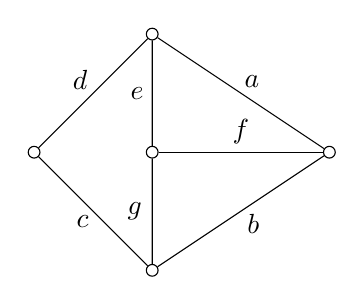
\begin{tikzpicture}[scale=1.5, every node/.style={circle, fill=white, draw, inner sep=1.5pt}]
        \node (left) at (0,1) {};
        \node (top) at (1,2) {};
        \node (mid) at (1,1) {};
        \node (bottom) at (1,0) {};
        \node (right) at (2.5,1) {};

        \draw (left) -- node[above left, draw=none, fill=none] {$d$} (top);
        \draw (left) -- node[below left, draw=none, fill=none] {$c$} (bottom);
        \draw (top) -- node[above right, draw=none, fill=none] {$a$} (right);
        \draw (bottom) -- node[below right, draw=none, fill=none] {$b$} (right);
        \draw (top) -- node[left, draw=none, fill=none] {$e$} (mid);
        \draw (mid) -- node[left, draw=none, fill=none] {$g$} (bottom);
        \draw (mid) -- node[above, draw=none, fill=none] {$f$} (right);
    \end{tikzpicture}
    \\ Figure 6.1
\end{center}

\begin{definition}[Edge Chromatic Number]
The \textbf{edge chromatic number} (or \textbf{chromatic index}) $\chi'(G)$ is the smallest number of colours required to properly colour the edges of $G$.
\end{definition}

\subsection{Basic Properties and Bounds}

\begin{itemize}
    \item \textbf{Lower bound:} 
    \[
    \chi'(G) \ge \Delta(G)
    \] 
    because the edges incident to a vertex of maximum degree must all have distinct colours.
    
    \item \textbf{Upper bound (Vizing's Theorem):} 
    \[
    \chi'(G) \le \Delta(G) + 1
    \]  
    This gives rise to the classification:
    \begin{itemize}
        \item \textbf{Class 1:} $\chi'(G) = \Delta(G)$
        \item \textbf{Class 2:} $\chi'(G) = \Delta(G)+1$
    \end{itemize}
\end{itemize}

\section{Vizing's Theorem}

\begin{theorem}[Vizing, 1964]
For any simple graph $G$:
\[
\Delta(G) \le \chi'(G) \le \Delta(G) + 1
\]
\end{theorem}

\begin{remark}
This theorem ensures that every simple graph can be edge-coloured using at most one more than the maximum degree of the graph.
\end{remark}

\subsection{Proof Sketch}
\begin{itemize}
    \item Colour edges sequentially.
    \item If no colour is available for a new edge, construct an \textbf{alternating path} between two colours.
    \item Swap colours along this path to free a colour.
    \item Repeat until all edges are coloured using at most $\Delta + 1$ colours.
\end{itemize}

\subsection{Examples}

\begin{example}[Bipartite Graph $K_{3,3}$]
$\Delta = 3$, $\chi'(K_{3,3}) = 3$ (Class 1)
\end{example}

\begin{example}[Complete Graph $K_5$]
$\Delta = 4$, $\chi'(K_5) = 5$ (Class 2)
\end{example}

\section{The Timetabling Problem}

\begin{definition}[Timetabling Problem]
Given a set of exams and students, schedule exams so that no student has overlapping exams.
\end{definition}

\subsection{Graph Theoretical Formulation}
\begin{itemize}
    \item Represent exams as vertices.
    \item Connect vertices with an edge if a student attends both exams.
    \item Each time slot corresponds to a colour in edge colouring.
    \item Construct the line graph $L(G)$ of the conflict graph $G$: vertices of $L(G)$ correspond to edges of $G$, adjacent if edges in $G$ share a vertex.
    \item Then $\chi(L(G)) = \chi'(G)$, reducing timetabling to edge colouring.
\end{itemize}

\section{K\"onig's Line Colouring Theorem}

\begin{theorem}[K\"onig, 1916]
For any bipartite graph $G$:
\[
\chi'(G) = \Delta(G)
\]
\end{theorem}

\begin{remark}
All bipartite graphs are Class 1. The theorem guarantees a proper edge colouring using exactly $\Delta(G)$ colours.
\end{remark}

\subsection{Proof Sketch}
\begin{itemize}
    \item Use induction on the number of edges.
    \item Apply Hall's Marriage Theorem to find matchings for each colour.
    \item Colour edges sequentially, ensuring no conflict at vertices.
\end{itemize}

\subsection{Example}
$K_{3,3}$ is bipartite with $\Delta = 3$, so by K\"onig's theorem, $\chi'(K_{3,3}) = 3$.

\section{Summary Table}

\begin{center}
\begin{tabular}{|>{\raggedright}p{3cm}|>{\raggedright}p{7cm}|>{\raggedright\arraybackslash}p{5cm}|}
\hline
\textbf{Concept} & \textbf{Definition / Statement} & \textbf{Notes} \\
\hline
Edge Colouring & Assignment of colours to edges so adjacent edges differ & Basis for chromatic index \\
\hline
Edge Chromatic Number ($\chi'$) & Minimum colours needed & $\Delta(G) \le \chi'(G) \le \Delta(G)+1$ \\
\hline
Vizing’s Theorem & $\chi'(G) \le \Delta(G)+1$ & Class 1 vs Class 2 \\
\hline
Timetabling Problem & Scheduling exams / tasks & Uses line graphs and edge colouring \\
\hline
K\"onig’s Line Colouring Theorem & $\chi'(G) = \Delta(G)$ for bipartite graphs & Always Class 1 \\
\hline
\end{tabular}
\end{center}

\section{Applications}

\begin{itemize}
    \item Scheduling problems (exams, tournaments, shifts)
    \item Register allocation in compilers
    \item Traffic flow management
    \item Frequency assignment in networks
\end{itemize}

\section{The Timetabling Problem}

\subsection{Problem Statement}

The \textbf{timetabling problem} models the scheduling of exams, classes, or tasks in such a way that no conflict occurs. Formally, consider:
\begin{itemize}
    \item $T$ teachers or instructors,
    \item $C$ classes or exams,
    \item A \textbf{teaching requirement matrix} $P = [p_{ij}]$, where $p_{ij}=1$ if teacher $i$ teaches class $j$, and $0$ otherwise.
\end{itemize}

We represent this problem as a \textbf{bipartite graph} $G = (T \cup C, E)$, where:
\begin{itemize}
    \item Vertices correspond to teachers $T$ and classes $C$.
    \item An edge $e=(t,c)$ exists if teacher $t$ teaches class $c$ (i.e., $p_{tc}=1$).
\end{itemize}

A \textbf{timetable} corresponds to an assignment of edges to \textbf{periods} such that:
\begin{itemize}
    \item No teacher is scheduled to teach more than one class in a period.
    \item No class is taught by more than one teacher in a period.
\end{itemize}

Equivalently, each period corresponds to a \textbf{matching} in the bipartite graph $G$, since matchings are sets of edges with no two edges incident to the same vertex.

\subsection{Balancing Matchings}

\begin{lemma}
Let $M$ and $N$ be disjoint matchings of $G$ with $|M| > |N|$. Then there exist disjoint matchings $M'$ and $N'$ of $G$ such that:
\[
|M'| = |M| - 1, \quad |N'| = |N| + 1, \quad \text{and } M' \cup N' = M \cup N.
\]
\end{lemma}

\textbf{Proof Sketch:}
\begin{itemize}
    \item Consider the subgraph $H = G[M \cup N]$, the union of edges in $M$ and $N$.
    \item Each component of $H$ is either:
    \begin{itemize}
        \item An even cycle, with edges alternating between $M$ and $N$, or
        \item A path with edges alternating between $M$ and $N$.
    \end{itemize}
    \item Since $|M| > |N|$, some path component $P$ must start and end with edges of $M$.
    \item Let $P = v_0 e_1 v_1 e_2 \cdots e_{2n+1} v_{2n+1}$. Then define:
    \[
    M' = (M \setminus \{ e_1, e_3, \dots, e_{2n+1} \}) \cup \{ e_2, e_4, \dots, e_{2n} \},
    \]
    \[
    N' = (N \setminus \{ e_2, e_4, \dots, e_{2n} \}) \cup \{ e_1, e_3, \dots, e_{2n+1} \}.
    \]
    \item This switches edges along the path, reducing $|M|$ by 1 and increasing $|N|$ by 1 while preserving disjointness.
\end{itemize}

\subsection{Theorem: Existence of $p$ Disjoint Matchings}

\begin{theorem}[]
Let $G$ be a bipartite graph with maximum degree $A$. If $p \ge A$, then there exist $p$ disjoint matchings $M_1, M_2, \dots, M_p$ of $G$ such that:
\begin{equation}
\bigcup_{i=1}^{p} M_i = E(G),
\end{equation}
\begin{equation}
\text{and any two matchings differ in size by at most one: } ||M_i| - |M_j|| \le 1.
\end{equation}
\end{theorem}

\textbf{Interpretation:} Each matching corresponds to a period in the timetable, so Theorem 6.3 guarantees:
\begin{itemize}
    \item Every edge (teacher-class assignment) is scheduled in some period.
    \item Workload is balanced across periods.
\end{itemize}

\subsection{Example: Teachers and Classes}

Suppose there are 4 teachers and 5 classes with the teaching requirement matrix $P$, and that one possible 4-period timetable is shown in Figure 6.4.

\begin{itemize}
    \item The edge decomposition of $G$ assigns edges to matchings:
    \begin{itemize}
        \item Normal edges $\to$ period 1,
        \item Broken edges $\to$ period 2,
        \item Wavy edges $\to$ period 3,
        \item Heavy edges $\to$ period 4.
    \end{itemize}
    \item Period 1 requires 4 rooms (4 edges in the matching). Total edges $|E| = 11$.
    \item By Theorem 6.3, a 4-period timetable can be arranged such that each period has either $\lceil 11/4 \rceil = 3$ or $\lfloor 11/4 \rfloor = 2$ classes.
\end{itemize}

\subsection{Refining the Timetable}

\begin{itemize}
    \item Let $M_1$ be the normal matching (period 1), $M_4$ the heavy matching (period 4), with $|M_1| = 4$ and $|M_4| = 2$.
    \item Consider $G[M_1 \cup M_4]$, which consists of two path components of length 3.
    \item Using Lemma 6.3, we can \textbf{swap edges along the paths}:
    \begin{itemize}
        \item Reduce $M_1$ by 1 edge and increase $M_4$ by 1 edge.
        \item Balance the matchings so each period has 2 or 3 classes.
    \end{itemize}
    \item This reduces the maximum number of rooms needed at any period from 4 to 3.
\end{itemize}

\begin{remark}
This procedure generalizes to any bipartite timetabling problem: given $p \ge \Delta(G)$ periods, the edges of the bipartite graph can be decomposed into $p$ disjoint matchings with roughly equal sizes, minimizing peak resource usage (e.g., rooms).
\end{remark}

% TO UPDATE
% --- FIGURE 6.4 ---
\begin{center}
    \begin{minipage}{0.45\textwidth}
        \centering
        \[
        P = 
        \begin{pmatrix}
        2 & 0 & 1 & 1 & 0 \\
        0 & 1 & 0 & 1 & 0 \\
        0 & 1 & 1 & 1 & 0 \\
        0 & 0 & 0 & 1 & 1
        \end{pmatrix}
        \]
        (a)
    \end{minipage}
    \begin{minipage}{0.45\textwidth}
        \centering
        \begin{tabular}{r|cccc|}
            \multicolumn{1}{c}{} & \multicolumn{4}{c}{Period} \\
            \multicolumn{1}{c}{} & 1 & 2 & 3 & 4 \\ \cline{2-5}
            $X_1$ & $Y_1$ & $Y_1$ & $Y_3$ & $Y_4$ \\
            $X_2$ & $Y_2$ & - & $Y_4$ & - \\
            $X_3$ & $Y_3$ & $Y_4$ & - & $Y_2$ \\
            $X_4$ & $Y_4$ & $Y_5$ & - & - \\ \cline{2-5}
        \end{tabular}
        \\[2mm] (b)
    \end{minipage}
    \\[0.5em] Figure 6.4
\end{center}

\[
\lfloor \epsilon/p \rfloor \leq |M_i| \leq \lceil \epsilon/p \rceil
\]

\vspace{2em}

% --- FIGURE 6.5 ---
\begin{center}
    \begin{minipage}{0.48\textwidth}
        \centering
        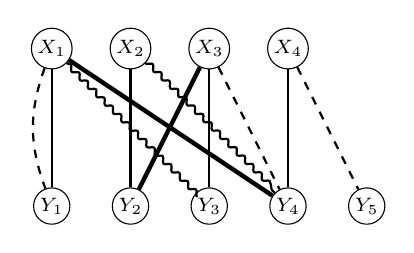
\begin{tikzpicture}[scale=1, every node/.style={circle, fill=white, draw, inner sep=1pt, font=\scriptsize}]
            \foreach \i in {1,...,4} \node (X\i) at (\i, 2) {$X_{\i}$};
            \foreach \j in {1,...,5} \node (Y\j) at (\j, 0) {$Y_{\j}$};
            % Figure 6.5(a) edges
            \draw[ultra thick] (X1)--(Y4) (X3)--(Y2);
            \draw[thick] (X1)--(Y1) (X2)--(Y2) (X3)--(Y3) (X4)--(Y4);;
            \draw[thick, dashed] (X1) to[bend right=20] (Y1);
            \draw[thick, dashed] (X3)--(Y4) (X4)--(Y5);
            \draw[thick, decorate, decoration={snake, amplitude=.3mm, segment length=1.5mm}] (X1)--(Y3) (X2)--(Y4);
        \end{tikzpicture}
        \\ (a)
    \end{minipage}
    \begin{minipage}{0.48\textwidth}
        \centering
        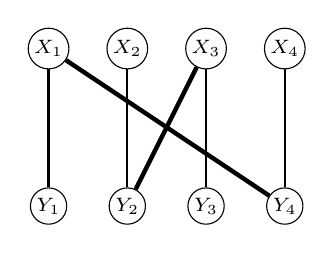
\begin{tikzpicture}[scale=1, every node/.style={circle, fill=white, draw, inner sep=1pt, font=\scriptsize}]
            \foreach \i in {1,...,4} \node (X\i) at (\i, 2) {$X_{\i}$};
            \foreach \j in {1,...,4} \node (Y\j) at (\j, 0) {$Y_{\j}$};
            % Figure 6.5(b) specific edges (Matchings M1 and M2)
            \draw[thick] (X1)--(Y1) (X2)--(Y2) (X3)--(Y3) (X4)--(Y4);
            \draw[ultra thick] (X1)--(Y4) (X3)--(Y2);
        \end{tikzpicture}
        \\ (b)
    \end{minipage}
    \\[0.5em] Figure 6.5
\end{center}

\vspace{2em}

% --- FIGURE 6.6 ---
\begin{center}
    \begin{minipage}{0.45\textwidth}
        \centering
        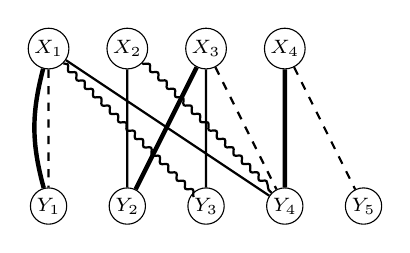
\begin{tikzpicture}[scale=1, every node/.style={circle, fill=white, draw, inner sep=1pt, font=\scriptsize}]
            \foreach \i in {1,...,4} \node (X\i) at (\i, 2) {$X_{\i}$};
            \foreach \j in {1,...,5} \node (Y\j) at (\j, 0) {$Y_{\j}$};
            % Edges matching the final coloring in Figure 6.6
            \draw[ultra thick] (X1) to[bend right=15] (Y1); 
            \draw[ultra thick] (X3)--(Y2) (X4)--(Y4);
            \draw[thick, dashed] (X1)--(Y1) (X3)--(Y4) (X4)--(Y5);
            \draw[thick] (X1)--(Y4) (X2)--(Y2) (X3)--(Y3);
            \draw[thick, decorate, decoration={snake, amplitude=.3mm, segment length=1.5mm}] (X1)--(Y3) (X2)--(Y4);
        \end{tikzpicture}
        \\ (a)
    \end{minipage}
    \begin{minipage}{0.45\textwidth}
        \centering
        \begin{tabular}{r|cccc|}
            \multicolumn{1}{c}{} & \multicolumn{4}{c}{Period} \\
            \multicolumn{1}{c}{} & 1 & 2 & 3 & 4 \\ \cline{2-5}
            $X_1$ & $Y_4$ & $Y_1$ & $Y_3$ & $Y_1$ \\
            $X_2$ & $Y_2$ & - & $Y_4$ & - \\
            $X_3$ & $Y_3$ & $Y_4$ & - & $Y_2$ \\
            $X_4$ & - & $Y_5$ & - & $Y_4$ \\ \cline{2-5}
        \end{tabular}
        \\[2mm] (b)
    \end{minipage}
    \\[0.5em] Figure 6.6 {Period order: (1)normal, (2)dash, (3)wiggle, (4)thick}
\end{center}

\end{document}

can u align and improve this code